\subsubsection{Implications of anti-nuclei measurements for cosmic-ray physics and dark-matter searches}
\label{sec:astro}

The HL-LHC physics program with \pp and \pPb collisions will allow for precision measurements of anti-nuclei production and related observables that have implications for cosmic-ray physics and dark-matter searches.
Cosmic-ray (CR) anti-nuclei \antip, \antid, and \antihethree~have long been considered as probes of new physics, such as dark matter annihilation~\cite{Donato:1999gy, Baer:2005tw, Donato:2008yx, Brauninger:2009pe, Kadastik:2009ts, Cui:2010ud, Dal:2012my, Ibarra:2012cc, Fornengo:2013osa, Carlson:2014ssa, Aramaki:2015pii,Korsmeier:2017xzj}. Detecting these particles is one of the main goals of various CR experiments (e.g. AMS-02 ~\cite{Giovacchini:2007dwa, kounineHebar}, GAPS~\cite{vonDoetinchem:2015zva, Aramaki:2015laa}, BESS-Polar \cite{Abe:2011nx}). 

The galaxy produces CR anti-nuclei as secondaries, due to collisions of CR protons and helium with interstellar matter. Information from accelerator experiments is essential for the theoretical description of the background constituted by these secondary anti-nuclei.
The flux of secondary anti-nuclei can be calculated with only minor sensitivity to the details of CR astrophysics. The point is to use secondary-to-secondary flux ratios, where astrophysical uncertainties largely cancel. 
%
Secondary \antip, \antid, and \antihethree~are all formed dominantly by the same set of reactions. 
%\footnote{The contribution from pHe is at the level of $\sim50\%$. Assuming that the branching fractions into $\ap,\,\ad,\,\ah$ are similar in pHe and \pp collisions (at the same $\sqrt{s}$/nuc), then our \pp-based analysis holds for pHe without modification.}: \pp. 
%
Using this basic fact, an explicit prediction for the locally observable flux of secondary \antid, relative to the flux of secondary \antip~can be derived~\cite{Ginzburg:1990sk,Katz:2009yd,Blum:2017qnn}:
%
\begin{eqnarray}
\label{eq:ad2ap}\frac{J_{\ad}(\R)}{J_{\ap}(\R)}&=&\frac{\int \rmd\epsilon\,J_{\mathrm{p}}(\epsilon)\,\frac{\rmd\sigma_{\mathrm{pp}\to\ad}(\epsilon,\epsilon_{\ad})}{\rmd\epsilon_{\ad}}}{\int \rmd\epsilon\,J_{\mathrm{p}}(\epsilon)\,\frac{\rmd\sigma_{\mathrm{pp}\to\ap}(\epsilon,\epsilon_{\ap})}{\rmd\epsilon_{\ap}}+\left(\sigma_{\ad}(\epsilon_{\ad})-\sigma_{\ap}(\epsilon_{\ap})\right)J_{\ap}(\R)}.
\end{eqnarray}
%
%
\noindent %Eq.~(\ref{eq:ad2ap}), the flux ratio on the left hand side is the theoretically predicted output, while the quantities on the right hand side are directly measurable quantities, that serve as the input for the prediction. 
Here $J_{\ad}(\R)$ is the predicted \antid~ flux, given at magnetic rigidity $\R = p/Z$, where $p$ is the momentum and $Z$ is the electric charge. $J_{\ap}(\R)$ is the (already well-measured~\cite{Aguilar:2016kjl}) \antip~ flux at the same rigidity, and  
%
$J_{\mathrm{p}}(\epsilon)$ is the proton flux~\cite{Aguilar:2015ooa} at energy $\epsilon$. 
%
$\frac{\rmd\sigma_{\mathrm{pp}\to\bar x}(\epsilon,\epsilon_{\bar x})}{\rmd\epsilon_{\bar x}}$ and $\sigma_{\bar x}(\epsilon_{\bar x})$ are the inclusive production and inelastic cross sections, respectively, with $x={\rm d},\,{\rm p}$. 
%This cross section is related to the Lorentz-invariant differential cross section, $\left(\epsilon\frac{d\sigma}{d^3p}\right)_{pp\to\ad}$, via
%%
%\begin{eqnarray}\label{eq:LICS}\frac{d\sigma_{pp\to\ad}(\epsilon,\epsilon_{\ad})}{d\epsilon_{\ad}}&=&2\pi \int_0^\pi d\theta\,p_t\, \left(\epsilon\frac{d\sigma}{d^3p}\right)_{pp\to\ad},\end{eqnarray}
%%
%where $\theta$ is the angle between the incoming proton and the outgoing secondary in the ISM frame.
%the analogous quantity for $\ap$ is $\frac{d\sigma_{pp\to\ap}(\epsilon,\epsilon_{\ap})}{d\epsilon_{\ap}}$. 
% 
%$\sigma_{\ad}(\epsilon_{\ad})$ and $\sigma_{\ap}(\epsilon_{\ap})$ are the energy-dependent inelastic cross sections for $\ad$ and $\ap$ on hydrogen. 
%In what follows, $\sigma_{\ad}(\epsilon)=2\,\sigma_{\ap}(\epsilon)$ is assumed.
% 
The particle energy $\epsilon_{\bar x}$ for a nucleus with mass number \Anucl is evaluated at $\R$: $\epsilon_{\ap}=\sqrt{\R^{2}+\mathrm{A}^2m_{\mathrm{p}}^{2}}$. 
%
To describe \antihethree~ we use an analogous expression to Eq.~(\ref{eq:ad2ap}), adding the production of $\at$ which decays to \antihethree. More details, including the relation of the differential cross section appearing in Eq.~(\ref{eq:ad2ap}) to the Lorentz-invariant differential cross section measurable at the LHC, can be found in~\cite{Blum:2017qnn}.
%

%No astrophysical CR propagation parameters or assumptions appear in Eq.~(\ref{eq:ad2ap}). 
%From the astrophysics point of view, Eq.~(\ref{eq:ad2ap}) amounts to the statement that the ratio of secondary CR fluxes measured locally, is equal to the ratio of their net\footnote{Net production $=$ (production) $-$ (inelastic loss).} production rates due to CR-ISM collisions. This prediction, valid for the description of secondary, stable, relativistic anti-nuclei, applies to all currently available CR propagation models~\cite{Ginzburg:1990sk,Katz:2009yd}. 
%
%Below, following~\cite{Blum:2017qnn}, we use Eq.~(\ref{eq:ad2ap}) to demonstrate the astrophysical implications of ALICE measurements. Recent calculations using a specific, detailed CR diffusion model~\cite{Korsmeier:2017xzj}, in which the $\ad$ and $\ah$ production cross section was also calibrated to match ALICE data, obtain results in agreement with ours. 

%Accelerator data is crucial to determine the anti-nuclei production cross section. 
The cross section for producing an anti-nucleus can be parameterized in terms of the anti-proton cross section, using the coalescence factor \BA: 
$(\epsilon_\mathrm{A}\rmd\sigma/\rmd^3p)_{\mathrm{pp}\to \mathrm{A}} = B_{\mathrm{A}}/\sigma_{\mathrm{pp}}^{\mathrm{A}-1} [(\epsilon_{\antip} \rmd\sigma/\rmd^3p)_{\mathrm{pp}\to \antip}]^\mathrm{A}$, 
where $\sigma_{\mathrm{pp}}$ is the total inelastic \pp cross section. 
Here, for simplicity, threshold effects are omitted~\cite{Duperray:2002pj,Duperray:2003tv,Blum:2017qnn}. 
%These effects cannot be measured from TeV-scale LHC data but are relevant for the astrophysical production: the integrals in Eq.~(\ref{eq:ad2ap}) receive contributions not far from the kinematic threshold. 
%Threshold correction as proposed in~\cite{Duperray:2002pj,Duperray:2003tv} and corrected in~\cite{Blum:2017qnn} can be further applied. 
%
Using Eq.~(\ref{eq:ad2ap}), and plugging in the coalescence factors experimentally obtained at the LHC~\cite{Acharya:2017fvb}, the predicted flux ratios can be obtained. 
%In~\cite{Blum:2017qnn}, coalescence model~\cite{Scheibl:1998tk} predictions for the $\overline{\rm d}$ and $\overline{^3\rm He}$ production cross section were given, consistent with subsequent LHC Run 1 data ~\cite{Acharya:2017fvb}. 
Secondary CR production is dominated by the low \pT\ region. As a result, the impact on the CR flux, due to \pT-dependent \BA, can be factored out to good approximation, allowing us to derive simple approximate formulae 
\footnote{Note that the rigidity $\mathcal{R}=100$~GV refers to the CR experiment rest frame, which is boosted w.r.t. the proton-proton collision centre of mass frame. In the proton-proton collision centre of mass frame, the anti-nuclei are formed close to threshold.}~\cite{Blum:2017qnn}:
%
\begin{eqnarray}\label{eq:J2}\frac{J_{\overline{\rm d}}\left(\R\right)}{J_{\overline{\rm p}}\left(\R\right)}\huge|_{\R=100{\rm GV}}&\approx&4\times10^{-4}\,\left(\frac{B_2}{1.5\times10^{-2}~\rm GeV^2}\right),\\%\end{eqnarray}
%
%
%\begin{eqnarray}
\label{eq:J3}\frac{J_{\antihethree}\left(\R\right)}{J_{\antip}\left(\R\right)}\huge|_{\R=100{\rm GV}}&\approx&2\times10^{-7}\,\left(\frac{B_3}{1.5\times10^{-4}~\rm GeV^4}\right),\end{eqnarray}
%
where, for CR studies, the $B_2$ and $B_3$ values should be read from the average yield in the range $\pT/\mathrm{A}=(0-0.5)~\gmom$ in the accelerator analysis. 
%
The precision requirements (O(10$\%$)) on the flux ratio determination for the astrophysical applications discussed here will be matched by measuring $B_{2}$ and $B_{3}$ in the lowest \pT\ bin with a relative systematic uncertainty of the order of 10$\%$ \cite{Acharya:2017fvb}. The latter largely dominates the statistical uncertainty that is expected to be of O(0.1$\%$)  already with \Lint~=~6~\pbInv in \pp collisions at $\sqrt{s}~=~5.5$~TeV. 
Moreover, a first measurement of $B_{4}$ in \pp collisions will be achievable in the same sample. The statistical precision on $B_{4}$ can be lowered to the 10$\%$ level if a luminosity of 200~\pbInv in \pp collisions at $\sqrt{s}~=~14$~TeV can be inspected with a dedicated trigger for (anti-)nuclei.

It is important to note that the \BA measurement~\cite{Acharya:2017fvb} performed by ALICE during the LHC Run 1 was confined to mid-rapidity, $|y|<0.5$. Possible $y$ dependence of the coalescence factor \BA at $y=\mathcal{O}(1)$, or variation of the \antip\ differential cross section with respect to current parameterisations~\cite{Donato:2017ywo}, would affect the prediction in Eqs.~(\ref{eq:J2}-\ref{eq:J3}). It would be an important task of future LHC measurements to test these effects. Similarly important, albeit -- possibly -- beyond the reach of the LHC, would be to study the low $\sqrt{s}=\mathcal{O}(10)$~GeV behaviour of \BA~\cite{Blum:2017qnn}.

\subsubsection{Implications of anti-nuclei measurements and hyperon-nucleon correlations for neutron star physics}

Although the neutron star crust is composed of neutrons, within the innermost core hyperons could be present \cite{RMP-88-035004-2016}.
Whether or not this scenario holds true depends on the two- and three-body hyperon nucleon interactions (YN and YNN) that are still only rather scarcely constrained experimentally.\\
At present the mass range for observed neutron stars is about (0.9 --  3.0)$M_{\bigodot}$ within errors \cite{ARNPS-62-485-2012}, where $M_{\bigodot}$ stands for the solar mass. 
The equation of state (EoS) of neutron stars is constrained by the mass-radius relationship, in particular, the maximum mass ($M_{\scriptsize{\mbox{max}}}$). An EoS with "conventional" (N$+\pi$) degrees of freedom provides $M_{\scriptsize{\mbox{max}}}$ invariably above 2$M_{\bigodot}$ \cite{HyperfineInteract-233-131-2015,Nature-467-1081-2010,AstrophysJ-832-167-2016}. 
However, adding the $\Lambda$ hyperon in the hadronic basis softens the EoS and, as a consequence, significantly reduces $M_{\scriptsize{\mbox{max}}}$. 
The solution of this so-called "hyperon puzzle" is non-trivial, and is presently the subject of very active research.

Thanks to the large yields of free hyperons and  exotic (anti-)hyper-nuclei that can be produced in collider experiments and the excellent particle identification capabilities of the ALICE experiment, the upcoming experimental campaigns in Runs 3 and 4 at the LHC offer a unique opportunity to quantitatively characterise hypermatter under controlled (laboratory) conditions and infer on the equation of state of compact objects as neutron stars.

One of the crucial  element to solve the ``hyperon puzzle'' is the determination of the $\Lambda$NN three-body forces. 
Calculations show that with a parameterization of these forces compatible with the hyper-nuclear binding energies, the admixture of $\Lambda$'s in neutron star matter gets strongly reduced such that the pressure to support a 2$M_{\bigodot}$ neutron star can be maintained \cite{Lonardoni:2014bwa}. 
The observation of neutron-rich $\Lambda$ hyper-nuclei like \hypfour\ etc. at colliders could be very promising for studying the effects of the
three-body $\Lambda$NN forces in dense strongly interacting matter since a precise knowledge of light neutron-rich hyper-nuclei energy level structure could imply far-reaching consequences for  dense strange stellar matter properties.

Another promising way to contribute to the understanding of the hyperon puzzle is to pin down the hyperon-nucleon two-body interaction
for hyperons such as $\Sigma^{-}$ and $\Xi^-$. These hyperons can also be produced within neutron rich matter 
(n + n $\rightarrow \Sigma^- +$ p, $\Lambda$ + n $\rightarrow \Xi^- +$ p) depending on their interaction with the surrounding neutrons.
Some models assume a repulsive p$\Sigma$ interaction and postulate that $\Sigma^{-}$ can appear in neutron rich matter only starting from baryon densities $\rho \simeq 4\rho_{0}$ (where $\rho_{0}$ is the density of standard nuclear matter) \cite{PRC-93-035808-2016}.
For $\Xi$, no reliable experimental information about the interaction is available.
Recent studies \cite{Acharya:2018gyz} showed that the femtoscopy technique applied to \pp and \pPb collisions at LHC energies are particularly suited to study the final state interaction between nucleons and strange baryons (e.g.: $\Lambda$--p) and between two strange baryons (e.g.: $\Lambda$--$\Lambda$). 
Indeed, small colliding systems such as \pp and \pPb lead to hadron sources of rather small dimensions, of the order of 1 fm, in the range where the strong interaction is mostly evident.
Also, the production mechanism of hadrons in minimum bias \pp and \pPb collisions is not affected by the intermediate creation of a QGP and its time-dependent evolution as in \PbPb collisions at LHC energies. This allows for a more precise study of the hadron-hadron interactions.

\begin{figure}
\centering
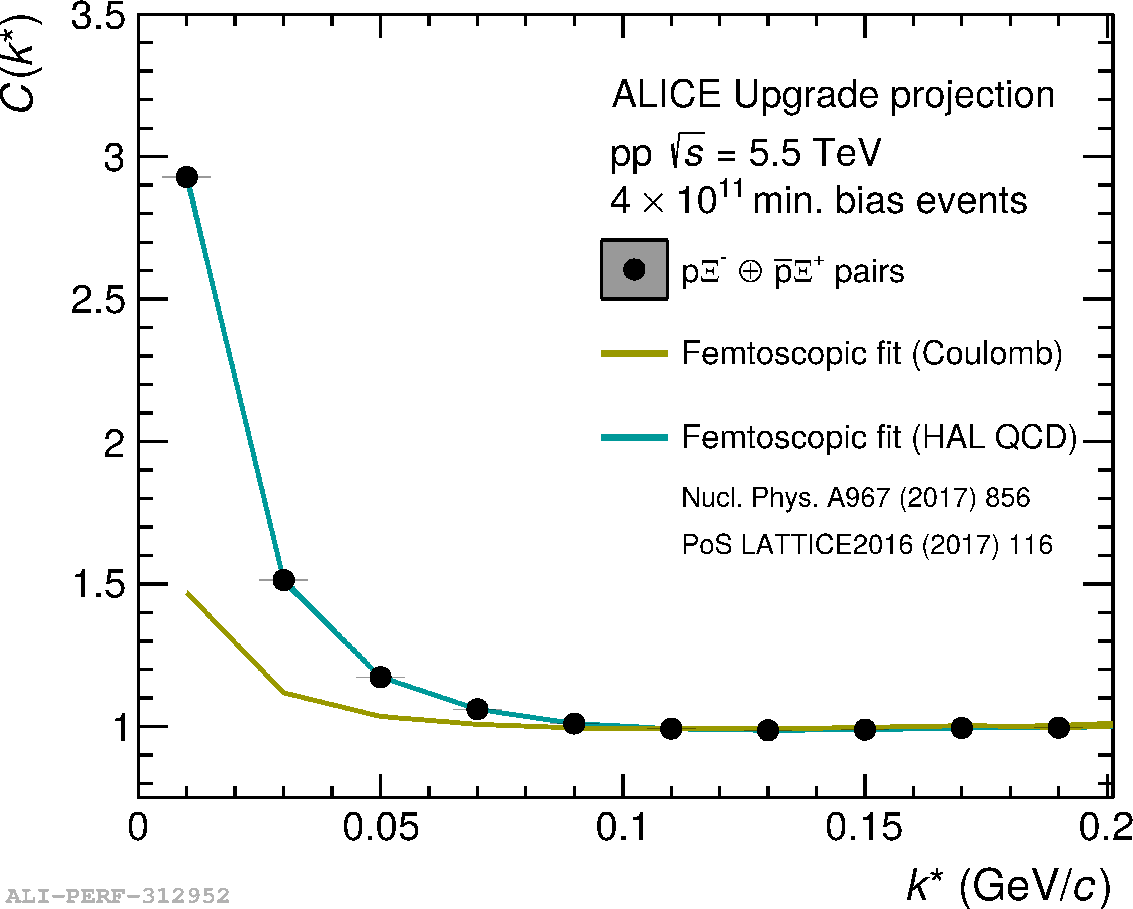
\includegraphics[width=.5\textwidth]{\main/lightflavour/figs/2018-11-15-2018-11-15-Projection_pXi_Model.pdf}
\caption{Expected p$\Xi^-$ + $\bar{\mathrm{p}}\Xi^+$ correlation for \pp collisions at $\sqrt{s} = 5.5$ TeV and $4\times 10^{11}$ minimum bias events, corresponding to \Lint~=~6~\pbInv. Only statistical errors have been considered.}
\label{pXiProj}
\end{figure}

Among the quantitative results obtained by ALICE in Run 2 at the LHC is the first observation of the attractive p$\Xi^-$ interaction \cite{alice-femto-inprep}.  
Figure \ref{pXiProj}  
shows the expected p$\Xi$ correlation for the Run 3 \pp sample as a function of the relative momentum $k*$. 
The projection is obtained on the basis of the current prediction by the HAL-QCD lQCD group \cite{Sasaki:2017ysy,Hatsuda:2017uxk} that is in agreement with the Run 2 results.
The clear deviation from the Coulomb-only correlation function shows the effect of the strong attractive interaction 
and the expected statistics will allow for a quantitative determination of the scattering parameters and the test of different hadronic models \cite{Haidenbauer:2018jvl,Rijken:2006kg}.
The investigation will also be extended to the $\Sigma^0$ hyperon, since in Run 3 and 4 we expect a total of 500,000 p$\Sigma^0$ pairs to be used to study the femtoscopy correlation.

In summary, massive neutron stars with $M \sim 2M_{\bigodot}$ are very intriguing recent observations in relativistic astrophysics. 
An improved account of the two-body YN interaction, the three-body $\Lambda$NN forces, and the contribution of multi-strange hyperons in the EoS is crucially important for more realistic description of compact astrophysical objects, in particular neutron and hybrid stars. The measurement of hyper-nuclei and hyperon correlations with the HL-LHC project are suggested as a promising tool for astrophysical applications.
